\documentclass[11pt]{article}
\usepackage{graphicx}
\usepackage{subfigure}
\usepackage[a4paper, total={6in, 8in}]{geometry}

% Title Page
\title{INF560 $\cdot$ Image Filtering}
\author{Delacourt Remi $\cdot$ Amponsem Kwabena}


\begin{document}
\maketitle
\newpage
\tableofcontents
\newpage

\section{Introduction}

In this project, parallel computation techniques were used to improve the performance of an image filtering program. In the sequential version, a GIF image is accepted as input and then an output, after filtering, is generated.
\begin{figure}[h]
	\centering
	\subfigure[]{
\includegraphics[scale=0.1]{images/original.png}}
	\subfigure[]{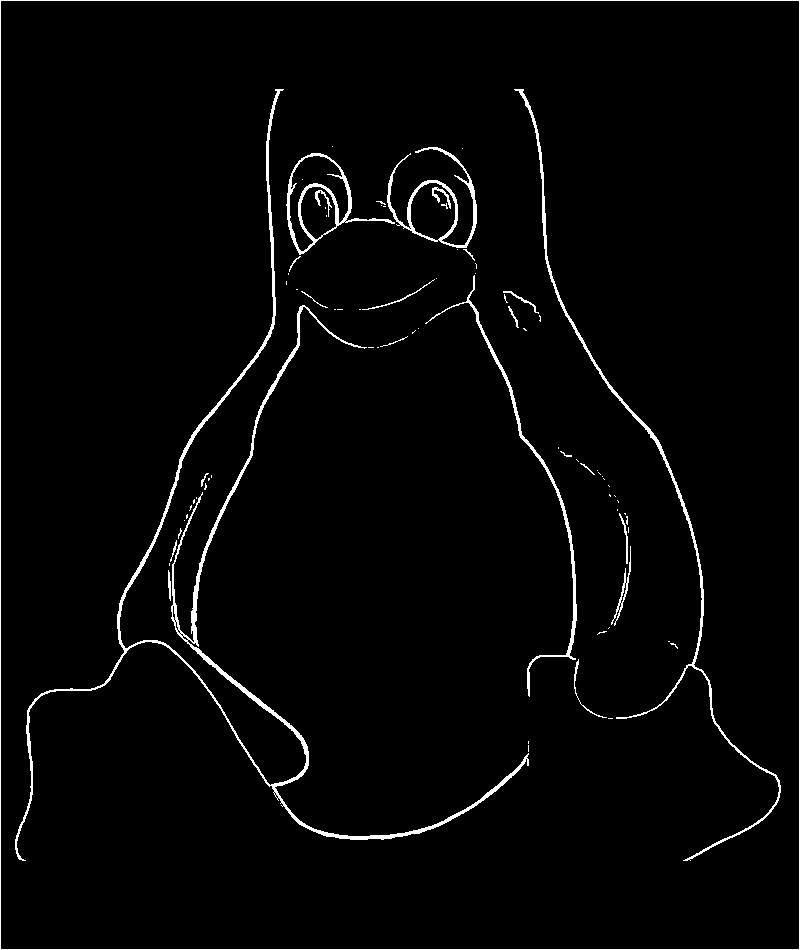
\includegraphics[scale=0.1]{images/processed.png}}
	\caption{(a) Original GIF image (b) Processed GIF image}
	\label{fig:introduction}
\end{figure}

To parallelize the sequential version, several parallelization models were studied and after vigorous investigation, one of the models were chosen.
\section{Overview}
Data parallelism is the type of parallelism employed in this project as it is the main focus of this module, INF560. 

The pixels of an animated GIF image are distributed in a fashion over all the processes. Initially, splitting animated GIF images into individual images was considered. 

At the first glance, that model seemed like the best option but after several iterations of critical thinking, it was noticed that the model only works best when there is an equal of amount of images as there are processes. Programming for such ideal cases had to be avoided at all cost since the application would be used in a real world environment where ideals are hard to achieve.

The report is structured as follows:
\begin{itemize}
	\item An in-depth explanation of the implementation of the parallel algorithm shown in Figure \ref{fig:overview} (considering MPI, OpenMP, and CUDA.)
	\item Performance evaluation juxtaposing the parallel version against the sequential version.
	\item A conclusion expressing how the objectives of the projects were achieved.
\end{itemize}
\begin{figure}[t!]
	\centering
	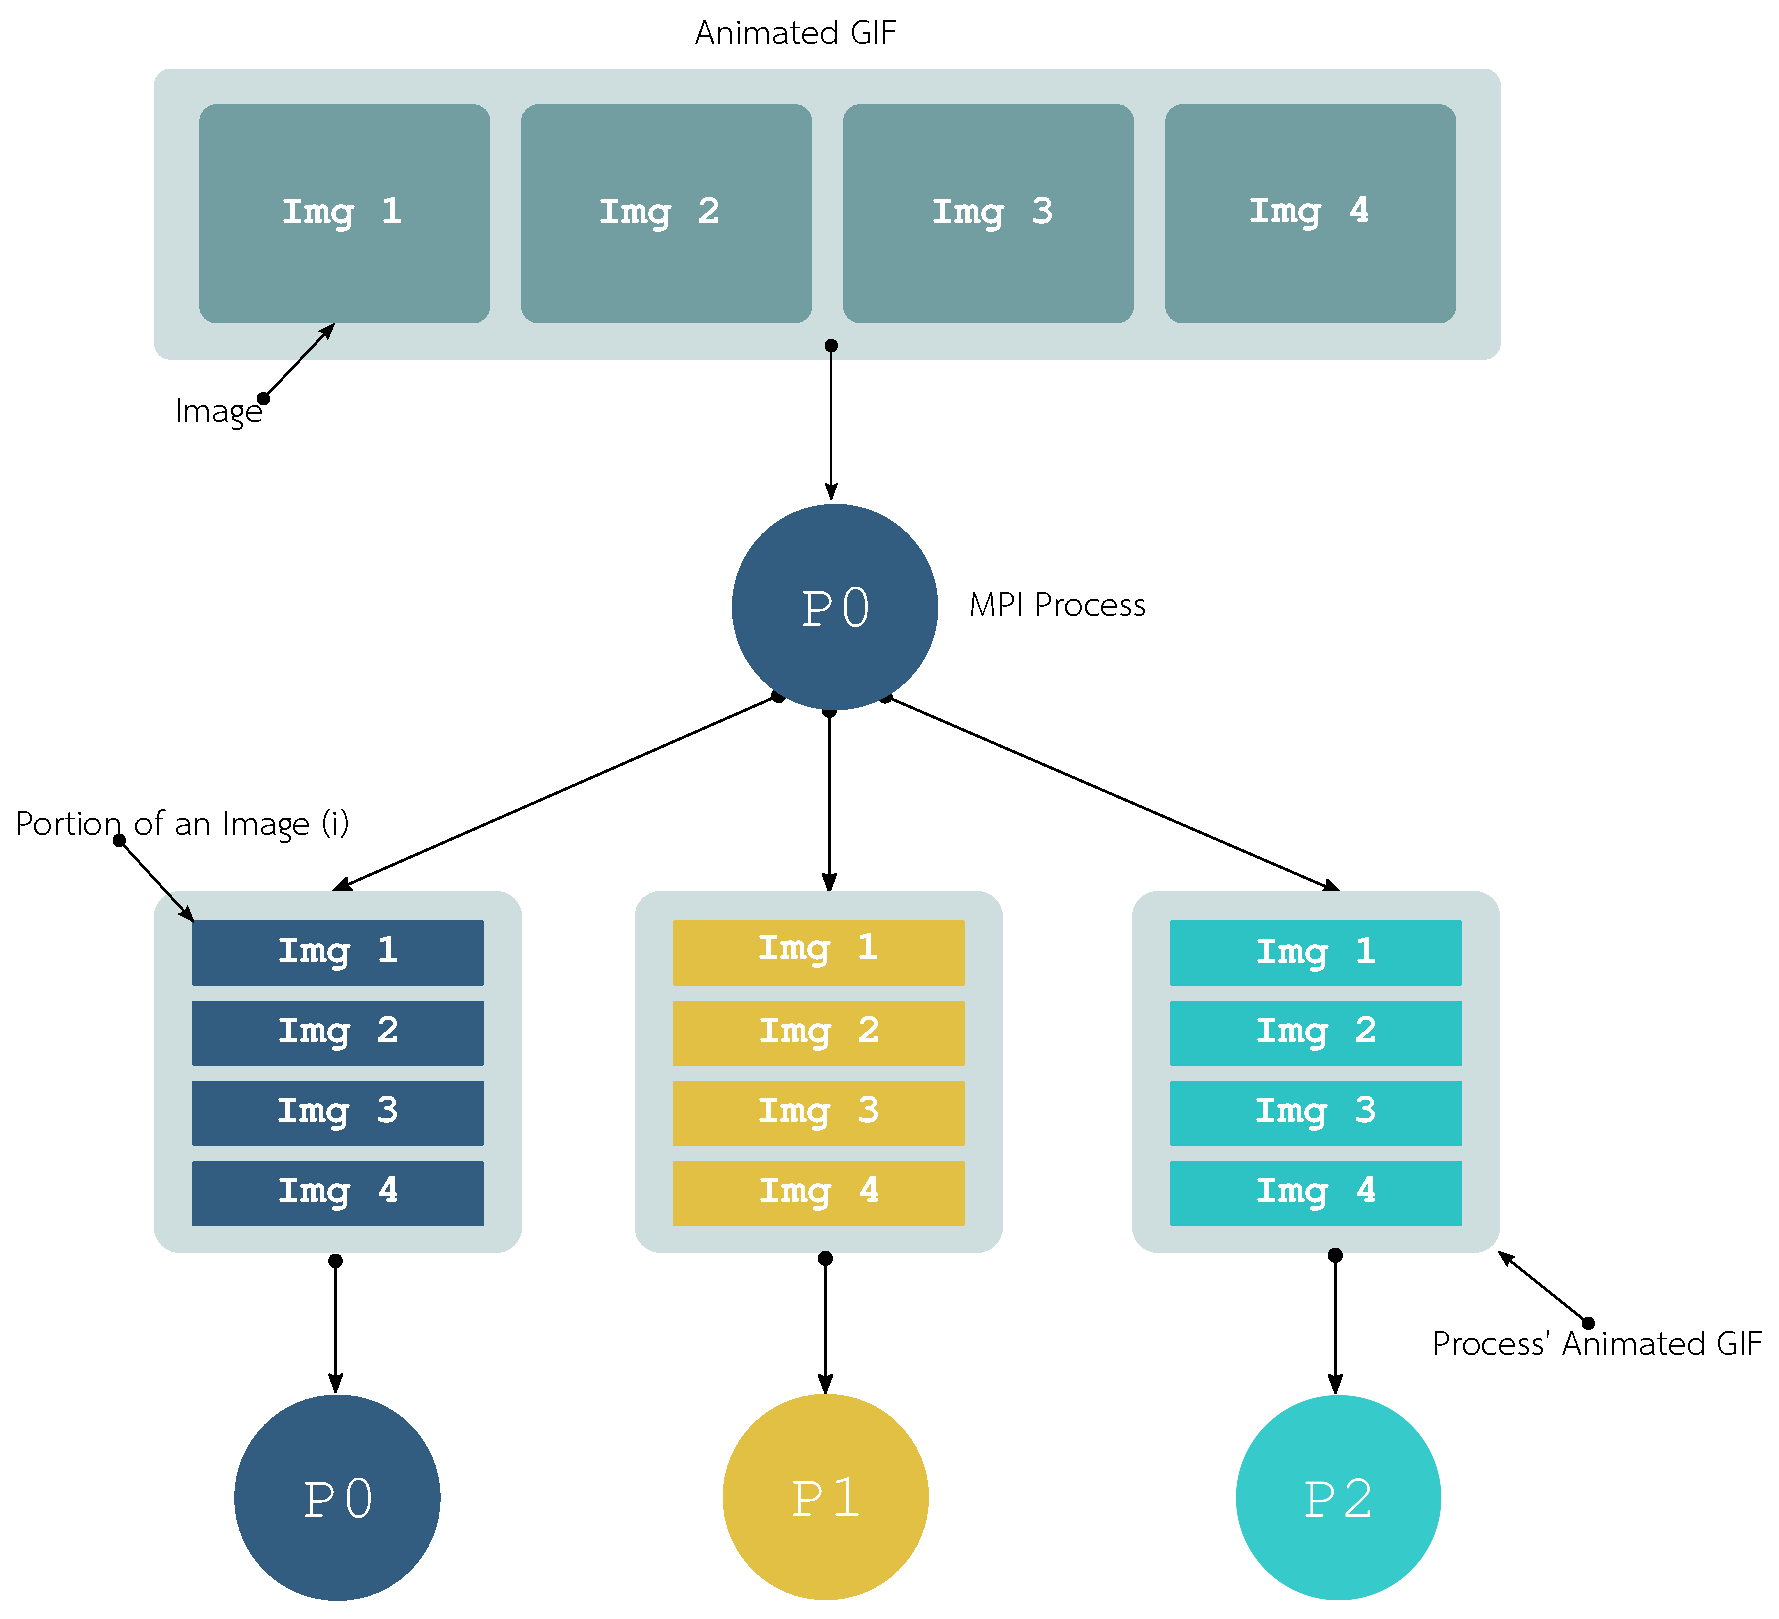
\includegraphics[scale=0.45]{INF560-Image-Filtering-EPS.eps}
	\label{fig:overview}
	\caption{High-level abstraction of the parallel algorithm.}
\end{figure}

\section{Implementation}

In this section, an in-depth explanation of the parallel algorithms employed in the project: how animated images were split up; how the images were recombined; how processing occurs on each process, is provided.

In our model, each image in the animated GIF is split according to the number of processes. This means that considering Figure \ref{fig:overview}, since there three (3) processes, each \textit{Img} would be divided into three portions along the height of the image, color coded as \textit{dark blue}, \textit{yellow}, and \textit{light blue}.

In that sense, each process would have a new animated image consisting of smaller chunks of all the individual images in the animated image.

\subsection{MPI}

The main focus of parallelism with MPI in this project is to parallelize computation and not I/O operations, and so, one process, \textbf{Process 0}, loads each animated GIF image and broadcasts its pixels to all the other processes.

Once a process receives the loaded pixels and metadata i.e., the number of individual images within the animated GIF, it then calculates the portion it has to work on. With this approach, each process calculates its own portion to work on.

\begin{figure}[h!]
	\centering
	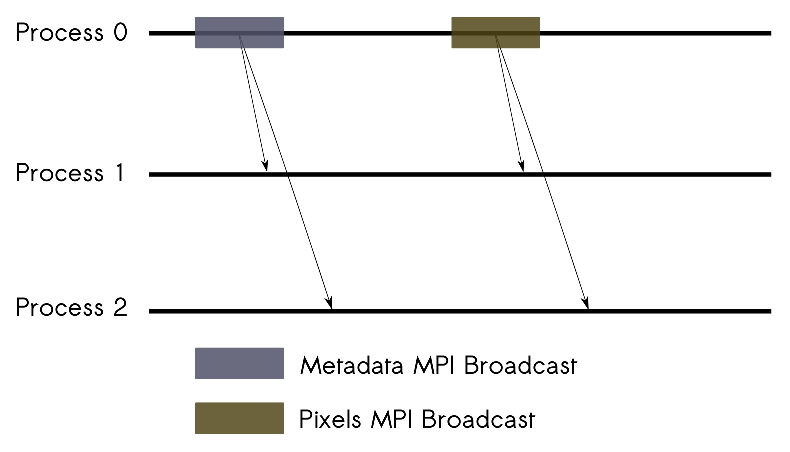
\includegraphics[scale=0.6]{MPI_Bcast.eps}
	\caption{The master process sending broadcasting data to other processes.}
\end{figure}
\subsection{OpenMP}
\subsection{CUDA}
\section{Evaluation}
\section{Conclusion}

In this project, several approaches were initially studied and then one i.e., the algorithm illustrated in Figure \ref{fig:overview}, was decided upon and implemented. And the results showed that the performance increased with increasing number of processes and threads.

This is the link to the GitHub repository of the project: 
\end{document}          
